Bei der Friedel-Crafts-Acylierung handelt es sich um eine elektrophile aromatische Substitution ($S_E\text{Ar}$) \cite{ROV}. 

Zunächst wird das Acetylchlorid durch die Lewis-Säure $\ce{AlCl3}$ aktiviert. 
Unter Abspaltung eines Chlorid-Ions entstehen ein stark elektrophiles Acylium-Ion und ein $\ce{AlCl4-}$-Komplex. 
Der nukleophile Angriff des $\pi$-Systems des Aromaten am Acylium-Ion hebt den aromatischen Zustand temporär auf und führt zur Bildung eines mesomeriestabilisierten Wheland-Komplexes. 

Die Rearomatisierung erfolgt durch Deprotonierung: 
Ein Chlorid-Ion des $\ce{AlCl4-}$ abstrahiert das Proton am $sp^3$-hybridisierten Ringkohlenstoff, wodurch unter Freisetzung von $\ce{HCl}$ das aromatische System wiederhergestellt wird. 
Da die basische Carbonylgruppe des entstandenen 2,4-Dimethylacetophenons einen stabilen Komplex mit dem $\ce{AlCl3}$ bildet, muss das Produkt im finalen Schritt durch wässrige Aufarbeitung zwingend hydrolytisch freigesetzt werden (Abb. \ref{fig:P1_M}).

\begin{figure}[H]
    \centering
    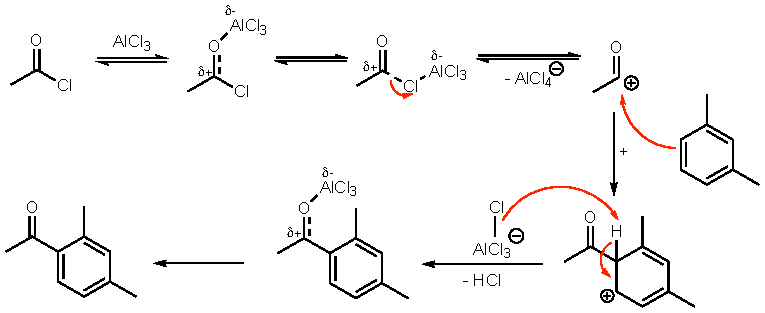
\includegraphics[width=1.0\textwidth]{drawings/P1_M.pdf} \\[0.5cm]
    \caption{Mechanismus der Friedel-Crafts-Acylierung von m-Xylol mit Acetylchlorid unter Aktivierung der Lewis-Säure Aluminiumchlorid im Lösungsmittel Dichlormethan.}
    \label{fig:P1_M}
\end{figure}